%%%%%%%%%%%%%%%%%%%%%%% file typeinst.tex %%%%%%%%%%%%%%%%%%%%%%%%%
%
% This is the LaTeX source for the instructions to authors using
% the LaTeX document class 'llncs.cls' for contributions to
% the Lecture Notes in Computer Sciences series.
% http://www.springer.com/lncs       Springer Heidelberg 2006/05/04
%
% It may be used as a template for your own input - copy it
% to a new file with a new name and use it as the basis
% for your article.
% 
% NB: the document class 'llncs' has its own and detailed documentation, see
% ftp://ftp.springer.de/data/pubftp/pub/tex/latex/llncs/latex2e/llncsdoc.pdf
%
%%%%%%%%%%%%%%%%%%%%%%%%%%%%%%%%%%%%%%%%%%%%%%%%%%%%%%%%%%%%%%%%%%%
   
\documentclass{llncs}

\usepackage{amssymb}
\setcounter{tocdepth}{3}
\usepackage{graphicx}
\usepackage{booktabs}
\usepackage{datatool}
\usepackage{tikz}
\usepackage{pgfplots}
\usepackage{pgfplotstable}
\usetikzlibrary{patterns}
\usepackage{lscape}
\usepackage{subfig}

\usepackage{url}
\urldef{\mailsa}\path|{alfred.hofmann, ursula.barth, ingrid.haas, frank.holzwarth,|
\urldef{\mailsb}\path|anna.kramer, leonie.kunz, christine.reiss, nicole.sator,|
\urldef{\mailsc}\path|erika.siebert-cole, peter.strasser, lncs}@springer.com|    
\newcommand{\keywords}[1]{\par\addvspace\baselineskip
\noindent\keywordname\enspace\ignorespaces#1}

\begin{document}

\mainmatter  % start of an individual contribution

% first the title is needed
\title{Can Data Integration Quality be Enhanced on Multi-cloud using SLA?}

% a short form should be given in case it is too long for the running head
%\titlerunning{Lecture Notes in Computer Science: Authors' Instructions}

% the name(s) of the author(s) follow(s) next
%
% NB: Chinese authors should write their first names(s) in front of
% their surnames. This ensures that the names appear correctly in
% the running heads and the author index.
% 
\author{
 Daniel A. S. Carvalho\inst{1},
 Pl\'acido A. Souza Neto\inst{3},  
        Genoveva Vargas-Solar\inst{4},
          Nadia Bennani\inst{2},
        Chirine Ghedira\inst{1}       
}
%
\authorrunning{Lecture Notes in Computer Science: Authors' Instructions}
% (feature abused for this document to repeat the title also on left hand pages)

% the affiliations are given next; don't give your e-mail address
% unless you accept that it will be published
\institute{Universit\'e Jean Moulin, Lyon 3 MAGELLAN, IAE -- France \\
			\email{daniel.carvalho@univ-lyon3.fr, chirine.ghedira-guegan@univ-lyon3.fr}
		\and
		CNRS INSA-Lyon, LIRIS, UMR5205 -- France\\
			\email{nadia.bennani@insa-lyon.fr}
		\and
		Instituto Federal do Rio Grande do Norte, Natal -- Brazil \\
			\email{placido.neto@ifrn.edu.br}
		\and
		CNRS, LIG-LAFMIA, Saint Martin d'H\`eres -- France \\
			\email{genoveva.vargas@imag.fr}
		}

%
% NB: a more complex sample for affiliations and the mapping to the
% corresponding authors can be found in the file "llncs.dem"
% (search for the string "\mainmatter" where a contribution starts).
% "llncs.dem" accompanies the document class "llncs.cls".
%

\maketitle

\begin{abstract}

\end{abstract}

\keywords{Systematic Mapping, Service Level Agreement, Data Integration, Multi-cloud Environment.}

% -------------------------------- Introduction -------------------------------- %
\section{Introduction}
\label{sec:intro}
The emergence of new architectures like the cloud opens new opportunities to data processing. 
The possibility of having unlimited access to cloud resources and the ``pay as U go'' model make it possible to change the hypothesis for processing big  data collections.  Instead of designing processes and algorithms taking into consideration  limitations on resources availability, the cloud sets the focus on the economic cost implied when using resources and producing results by parallelizing their use while delivering data under subscription oriented cost models.
 
Integrating and processing heterogeneous Big Data calls for efficient methods for correlating, associating, filtering them taking into consideration their ``structural'' characteristics (due to data variety) but also their quality (veracity), e.g., trust, freshness, provenance, partial or total consistency. 
Existing data integration techniques need to be revisited considering weakly curated and modeled data sets provided by different services under different quality conditions. Data integration can be done according to  (i) quality of service (QoS) requirements expressed by their consumers and (ii) Service Level Agreements (SLA)  exported by the cloud providers that host  Big Data and deliver resources for executing the associated management processes. Yet, it is not an easy task to completely enforce SLAs particularly because consumers use several cloud providers to store, integrate and process the data they require under the specific conditions they expect.
Naturally, a collaboration between cloud providers becomes necessary~\cite{036} but this should be also done in a user-friendly way, with some degree of transparency. 

  %Particularly, for queries that call several services deployed  on different clouds.

%\subsection{Contribution}
Data integration has to be revisited according to  the properties of data collections (volume, variety, velocity), to service oriented data provision contexts normally done in the context of cloud environments. Such environments (multi-cloud)  provide the required storage, computing and processing resources but they call for new strategies for integrating data considering different SLAs, subscription conditions, and data consumption requirements and preferences. In this context, the contribution of our work is two-fold. First it proposes a classification scheme of existing works fully or partially addressing the problem of integrating data in multi-cloud environments eventually taking into consideration Service Level Agreement. Second, the description of our vision  for guiding data integration in multi-cloud environments  by SLA and user/applications preferences. 

The classification scheme results from  applying the  methodology defined in~\cite{SM:Petersen:2008} called  \textit{systematic mapping}  for defining a classification of a field. A classification consists of categories clustered into facets in which publications (i.e., papers) are aggregated according to frequencies (i.e., number of published papers). According to the methodology, the study consists in  five interdependent tasks including (i) the definition of a research scope by defining research questions; (ii) retrieving candidate papers by querying different scientific databases (e.g. IEEE, Citeseer, DBLP); (iii) selecting relevant papers that can be used for answering the research questions by defining inclusion and exclusion criteria; (iv) defining a classification scheme by analyzing the abstracts of the selected papers to identify the terms that will be used as categories for classifying the papers; (v) producing a systematic mapping by sorting papers according to the classification scheme. 

Our final objective by applying the systematic mapping methodology is to identify trends and open issues regarding data integration in multi-cloud environments. Thus, our classification scheme consists in four facets that classify existing scientific publications addressing  together or independently SLA, Data Integration in Multi-cloud environments. We define two additional facets to identify the type of papers (e.g., position, survey, etc) and the type of contribution (e.g., model, architecture, system). It shows the research trends of data integration as a result of the emergence of the cloud and the characteristics associated to Big Data processing. The study and the classification scheme that we propose support  the proposal of our vision for filling some gaps and propose an original data integration solution according to current trends in the area. 


%\subsection{Organization of the paper}
The remainder of this paper is organized as follows. 
Section~\ref{sec:sm} describes our study of  data integration perspectives and the evolution of the research works that address some aspects of the problem. The section gives a quantitative analysis of our study and identifies open issues in the field. Section \ref{sec:approach} gives the general lines of the approach we propose for guiding data integration using SLA agreements in a multi-cloud environment.  Section~\ref{sec:rw} discusses existing approaches studying data integration problems in multi-cloud contexts that take into account SLA contacts.
Section~\ref{sec:conc} concludes the paper and discusses future work. 


 
% --------------------------------              -------------------------------- %
 
%. . . . . . . . . . . . . . . . . . . . . . . . . . . . . . . . . . . . . . . . . . . . . . . . . . . . . . . . . . . . . . . . . . . . . . . . . . . . . . . . . . . . 
\section{Data integration challenges: classification scheme}\label{sec:sm}
%. . . . . . . . . . . . . . . . . . . . . . . . . . . . . . . . . . . . . . . . . . . . . . . . . . . . . . . . . . . . . . . . . . . . . . . . . . . . . . . . . . . . 

The aim of our bibliographic study using the systematic mapping methodology \cite{SM:Petersen:2008} is to (i) categorize and quantify the key contributions and the evolution of the research done on \textit{SLA-guided
data integration in a multi-cloud environment} and  (ii) discover open issues and limitations of existing works.    
Our study is guided by  three research questions:


\textit{\textbf{RQ1:} Which are the SLA measures that have been mostly
applied  in the cloud?} This question  identifies  the type of
properties used for characterizing and evaluating the services provided  by
different clouds.   
 
\textit{\textbf{RQ2:}  How have published papers on data
 integration evolved towards cloud topics?} This question is devoted to identify the way  data integration problems addressed in the literature started  to include issues introduced by the cloud.

\textit{\textbf{RQ3:} In which way and in which  context has data integration  been linked to Quality of Service (QoS) measures in the literature?} The objective of this question is to understand which QoS measures have been used for evaluating data integration and to determine the conditions in which  specific measures are particularly used.

%--------------------------------------------------------------------------------------------------------------------------------------------
\subsection{Searching and screening  papers} \label{subsec:search}
%--------------------------------------------------------------------------------------------------------------------------------------------

According to our research questions and our expertise in data integration we chose a set of keywords to define a complex query to be used for retrieving papers from four target publication databases: IEEE~\footnote{http://ieeexplore.ieee.org/},
ACM~\footnote{http://dl.acm.org/}, Science Direct~\footnote{http://www.sciencedirect.com/} and
CiteSeerX~\footnote{http://citeseerx.ist.psu.edu/}. We used the following conjunctive and disjunctive general query which was completed with associated terms from a thesaurus and rewritten according to the expression rules of advanced queries in each database: 




\begin{center}
\textit{("Service level agreement"  AND ("Data integration" OR "Database
integration") AND ("Cloud" OR "Multi-cloud "))} \\
\end{center}
\medskip  

We retrieved  a total of 1832 publications. As a result of the filtering process
proposed by the systematic mapping methodology~\cite{SM:Petersen:2008} we excluded 1718 publications.
The number of papers included for building the final collection were 114
publications~\footnote{List of references available in:
https://github.com/danielboni/DEXA-2015-Can-Data-Integration-Quality-be-Enhanced-on-Multi-cloud-using-SLA.git}.

%--------------------------------------------------------------------------------------------------------------------------------------------
\subsection{Defining classification facets}
%--------------------------------------------------------------------------------------------------------------------------------------------

We analyzed the titles and abstracts of the  papers derived in the previous
phase using information retrieval techniques  to identify  frequent
 terms. We used these terms for proposing a classification scheme
consisting of three facets that group dimensions. The following lines define the facets and dimensions of the
classification scheme we propose. 

%.  -   .  .  -   ..  -   ..  -   ..  -   ..  -   ..  -   ..  -   ..  -   ..  -   ..  -   ..  -   ..  -   ..  -   ..  -   ..  -   ..  -   ..  -   ..  -   ..  -   ..  -   ..  -   ..  -   ..  -   .  
\textbf{\textit{Data Integration Environment:}}  
%.  -   .  .  -   ..  -   ..  -   ..  -   ..  -   ..  -   ..  -   ..  -   ..  -   ..  -   ..  -   ..  -   ..  -   ..  -   ..  -   ..  -   ..  -   ..  -   ..  -   ..  -   ..  -   ..  -   ..  -   .  
This facet groups the dimensions that characterize the architectures used for delivering data integration services ({\em data warehouse} and  {\em federated database}) and  architectures used for deploying these services ({\em cloud} and {\em multi-cloud}).

%.  -   .  .  -   ..  -   ..  -   ..  -   ..  -   ..  -   ..  -   ..  -   ..  -   ..  -   ..  -   ..  -   ..  -   ..  -   ..  -   ..  -   ..  -   ..  -   ..  -   ..  -   ..  -   ..  -   ..  -   .  
\textbf{\textit{Data Integration Description:}}
%.  -   .  .  -   ..  -   ..  -   ..  -   ..  -   ..  -   ..  -   ..  -   ..  -   ..  -   ..  -   ..  -   ..  -   ..  -   ..  -   ..  -   ..  -   ..  -   ..  -   ..  -   ..  -   ..  -   ..  -   .  
 This facet groups the dimensions describing the approaches used for describing the databases content in order to  integrate them. Data integration can be done by using {\em meta-data, schema}, and {\em knowledge}.

%.  -   .  .  -   ..  -   ..  -   ..  -   ..  -   ..  -   ..  -   ..  -   ..  -   ..  -   ..  -   ..  -   ..  -   ..  -   ..  -   ..  -   ..  -   ..  -   ..  -   ..  -   ..  -   ..  -   ..  -   .  
\textbf{\textit{Data Quality:}} 
%.  -   .  .  -   ..  -   ..  -   ..  -   ..  -   ..  -   ..  -   ..  -   ..  -   ..  -   ..  -   ..  -   ..  -   ..  -   ..  -   ..  -   ..  -   ..  -   ..  -   ..  -   ..  -   ..  -   ..  -   .  
This facet groups the dimensions  representing data quality measures. Measures can be related directly to data for instance {\em confidentiality, privacy, security, protection and provenance} and to the conditions in which data is integrated and delivered  (i.e., dimension {\em SLA}).           

The original vision of our classification scheme is that of adding the notion of {\em quality} to data integration represented by the facets {\em data quality}
and  {\em SLA}.
With these facets our classification scheme shows the aspects that must be considered when addressing data integration in the cloud  taking into account (i) the quality of data, (ii) the systems that integrate data and (iii) the quality warranties that a data consumer can expect expressed in SLAs.

%------------------------------------------------------------------------------- %
\section{Quantitative Analysis}\label{sec:qanalysis}
%--------------------------------------------------------------------------------% 

This section discusses the quantitative analysis  presented in bubble charts that combine different facets. 
In order to observe the evolution of the publication trends we defined a time screen between the years 1998 and 2014 (see Figure \ref{fig:pubperyear}). SLA has emerged when Cloud issues started to be addressed around 2009. The number of publications has increased as cloud infrastructures have become more popular and accessible. It seems  that data integration is an open issue when it is combined with SLA and cloud trends. Less recent papers seem to be devoted to the way data is described under schemata or knowledge representation strategies. This could be due to the fact that these strategies are consolidated today and  to the emergence of NoSQL approaches with their schema-less philosophy \cite{sadalage2012nosql}. 

\begin{figure}[ht!]
\centering
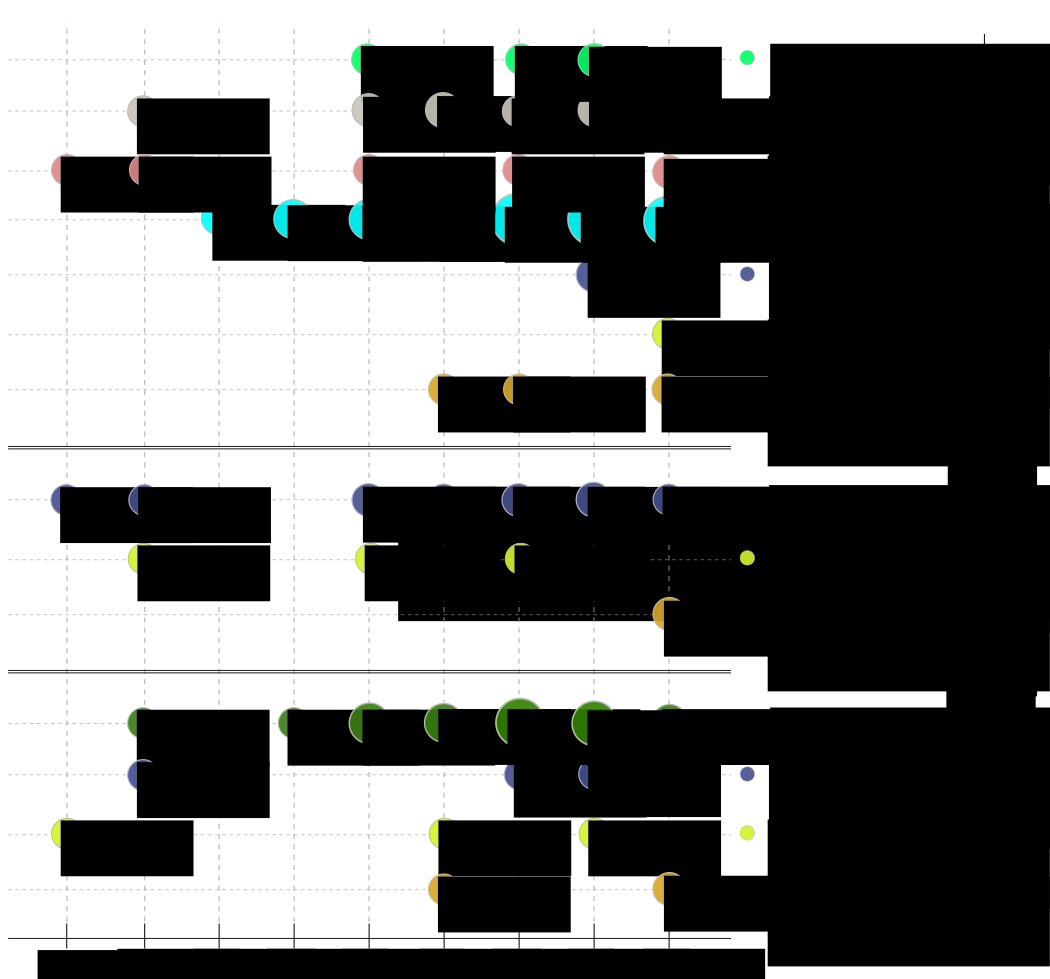
\includegraphics[scale=0.33]{figs/bubble-charts/PublicationsPerYear.pdf} 
\caption{Publications Per Year}\label{fig:pubperyear}
\end{figure}

We combined facets for answering the research questions proposed for guiding our
study. The following lines discuss the answers.
 
%  . .  .  . .  .  . .  .  . .  .  . .  .  . .  .  . .  .  . .  .  . .  .  . .  .  . .  .  . .  .  . .  .  . .  .  . .  .  . .  .  . .  .  . .  .  . .  .  . .  .  . .  .  . .  .
\textbf{\textit{RQ1: Which are the SLA measures that have been mostly applied 
in the cloud?}}
%  . .  .  . .  .  . .  .  . .  .  . .  .  . .  .  . .  .  . .  .  . .  .  . .  .  . .  .  . .  .  . .  .  . .  .  . .  .  . .  .  . .  .  . .  .  . .  .  . .  .  . .  .  . .  .


The facets SLA expression, data integration description and contribution give elements for determining which SLA measures have been applied to the cloud (Figure~\ref{fig:facet1}). 
The resulting bubble chart shows that most contributions propose SLA models and that  \textit{privacy}
and \textit{security} (11 papers - 9.65\%) are the most popular measures considered by SLA models for the cloud. These measures concern the network, information, data protection and confidentiality in the cloud. Most contributions propose SLA models (53 papers - 46.49\%)  but some languages (8 papers - 7.02\%) have also emerged. {\em Data provenance} is also a measure that emerges but only in papers dealing with multi-cloud environments. Data integration is merely addressed by using schemata (12 papers - 10.53\%)  and meta-data (4 papers - 3.51\%) particularly through models (34 papers - 29.82\%) and tools (25 papers - 21.93\%). Still, some works propose surveys (8 papers - 7.02\%).
 
\begin{figure}[ht!]
\centering
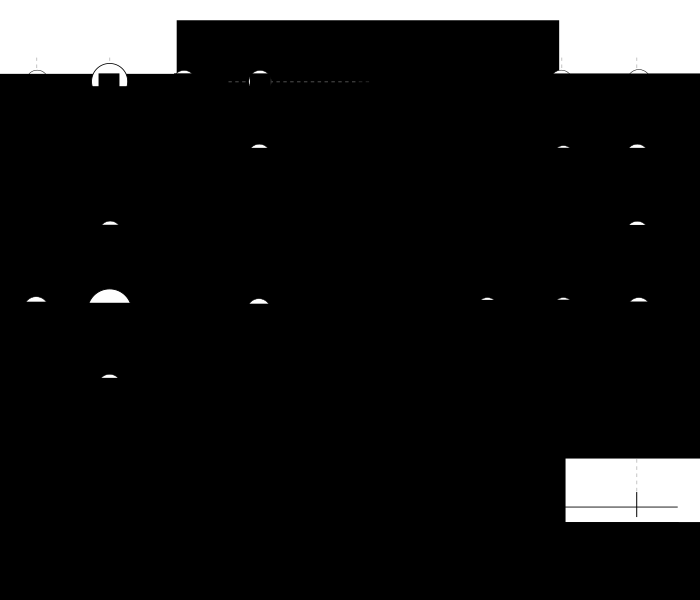
\includegraphics[width=0.75\textwidth]{figs/bubble-charts/Contribution-SLA-DIdescription.pdf}
  
\caption{Facets Contribution, SLA and Data Integration Description}\label{fig:facet1}
\end{figure} 

%  . .  .  . .  .  . .  .  . .  .  . .  .  . .  .  . .  .  . .  .  . .  .  . .  .  . .  .  . .  .  . .  .  . .  .  . .  .  . .  .  . .  .  . .  .  . .  .  . .  .  . .  .  . .  .
\textbf{\textit{RQ2: How have published papers on data integration evolved towards cloud topics?}}
%  . .  .  . .  .  . .  .  . .  .  . .  .  . .  .  . .  .  . .  .  . .  .  . .  .  . .  .  . .  .  . .  .  . .  .  . .  .  . .  .  . .  .  . .  .  . .  .  . .  .  . .  .  . .  .
\begin{figure}[h]
\centering
\includegraphics[width=0.86\textwidth]{figs/bubble-charts/DI-Environment-Contribution-Research.pdf}
\caption{Facets Data Integration Environment, Contribution and Research}\label{fig:facet2}
\end{figure}

Combining the facets data integration environment, contribution
and research it is possible to observe  the evolution of publications on data integration towards the cloud (Figure~\ref{fig:facet2}).  {\em Data warehouse} environments are the most common architecture. This can be explained by the increase of scientific  and industrial applications needing to build integrated  data sets for performing analysis and decision making tasks. The proposals are delivered as {\em models}  (14  papers - 12.27\%)  and {\em tools} (18
papers - 15.78\%)  used for facilitating data integration, mostly done in the {\em cloud}.  The most popular deployment environment of recent papers is the {\em cloud}. Given the importance and crucial need of data integration  most papers present concrete solutions as algorithms, methods and systems (31 papers - 27.19\%).
  
%  . .  .  . .  .  . .  .  . .  .  . .  .  . .  .  . .  .  . .  .  . .  .  . .  .  . .  .  . .  .  . .  .  . .  .  . .  .  . .  .  . .  .  . .  .  . .  .  . .  .  . .  .  . .  .
\textbf{\textit{RQ3:  In which way and in which context has data integration been linked to QoS measures in the literature?}}
%  . .  .  . .  .  . .  .  . .  .  . .  .  . .  .  . .  .  . .  .  . .  .  . .  .  . .  .  . .  .  . .  .  . .  .  . .  .  . .  .  . .  .  . .  .  . .  .  . .  .  . .  .  . .  .
\begin{figure}[!h]
\centering
\includegraphics[width=0.85\textwidth]{figs/bubble-charts/Data-Quality-DI.pdf}
\caption{Facets Data Quality, Data Integration Environment and Data Integration Description}\label{fig:facet4}
\end{figure}

We answered RQ3 by combining the facet {\em data quality} with the facets {\em data integration environment} and {\em data integration description}
(Figure~\ref{fig:facet4}).  Data integration and QoS measures are associated within environments like cloud  (9.68\%) and multi-cloud (4.39\%).

According to our quantitative analysis we observe that QoS has started to be
considered for integrating data. 
 The cloud is becoming a popular environment to
perform data integration in which security issues are most frequently addressed.
We identify a promising research area concerning the need of studying SLA which
is currently addressed  for the cloud as a whole \cite{PedrinaciCL14} but that
needs to be specialized for data integration aspects. Therefore, it is important
to identify the measures that characterize the quality of data and  the
quality measures associated to different phases of data integration. These phases include selecting
data services, retrieving data, integrating and correlating them and building a
query result that can be eventually stored and that must be delivered. The data integration phases are implemented by greedy algorithms and generate intermediate data that
can be stored for further use. Therefore they consume storage, computing,
processing and communication resources that have an associated economic cost. These resources 
 must ensure some QoS guarantees to data consumers. This problem seems to be
open in the domain, and we believe that it must be part of  a new vision of data
integration. We believe that it is possible to add and enhance the quality of
data integration by including SLAs.                   
 

\section{Conclusion and final remarks}\label{sec:conc}
This paper introduces the challenge of integrating data from distributed data
services deployed on different cloud providers guided by SLAs and user preferences statement. The data integration problem
is stated as a continuous data provision problem that has associated SLAs and
that uses techniques for ensuring different qualities of delivered data
(freshness, precision, completeness). The problem statement was derived from a
classification scheme that resulted from a study of existing publications
identified by applying the systematic mapping method. 
Our contribution is the definition of a classification scheme that shows the
aspects that characterize a modern vision of data integration done in
multi-cloud environments and that can be enhanced by including SLAs in its
process.  

Current big data settings impose to consider SLA and different data delivery
models. Given the volume and the complexity of query evaluation
that includes steps that imply greedy computations, it is important to combine
and revisit well-known solutions.

From the results of our systematic analysis,  we identified trends and open
issues in our research topic and proposed the general lines of an original data integration solution.  We are also  developing the strategies to
better define a SLA extension and data consumers preferences description for
guiding data integration in multi-cloud environments.
      

\bibliographystyle{plain}
\bibliography{bibliography,biblio,example}


\end{document}